\documentclass{article}
\usepackage{amsmath}
\usepackage{graphicx}
\usepackage{listings}
\usepackage{xcolor}
\usepackage{amsmath}
\usepackage{amssymb}
\usepackage{hyperref}
\usepackage{graphicx}
\usepackage{tikz}
\usepackage{geometry}
\usepackage{tcolorbox}
\geometry{margin=0.6in} % margins (default is ~1.5-1.75in)
\usetikzlibrary{positioning}

\usepackage{xcolor} % for dark mdoe
% \definecolor{dark}{HTML}{1F1F1F}
% \pagecolor{dark}
% \color[rgb]{1,1,1}

%%% >>> MY INFORMATION >>>
%%% Name: Kiarash Sotoudeh
%%% Student ID: 1010052194
%%% Email: kiarash.sotoudeh@mail.utoronto.ca
%%% <<< MY INFORMATION <<<

\definecolor{navyblue}{rgb}{0.0, 0.0, 0.5}
\definecolor{myblue}{RGB}{20, 80, 220}
\definecolor{answer}{RGB}{0, 20, 180}


\title{CSC311: Assignment 1 Writeup}
\author{Kiarash Sotoudeh}
\date{} 

% custom colors for code elements
\definecolor{codekeyword}{rgb}{0.0, 0.0, 0.6}
\definecolor{codecomment}{rgb}{0.0, 0.5, 0.0}
\definecolor{codestring}{rgb}{0.6, 0.0, 0.0}

% the listings package
\lstset{
  language=C,                      % language C  
  basicstyle=\ttfamily\small,      % font type and size
  keywordstyle=\color{codekeyword}\bfseries, % keyword color and style
  commentstyle=\color{codecomment}\itshape,  % comment color and style
  stringstyle=\color{codestring},  % string literal color
  numbers=left,                    % line numbers on the left
  numberstyle=\tiny\color{gray},   % line number style
  frame=single,                    % a frame around the code
  breaklines=true,                 % line breaking
  backgroundcolor=\color{white},   % background color
  tabsize=4,                       % tab size
  showspaces=false,                
  showstringspaces=false           
}

\begin{document}

\maketitle

\section*{Question 1}
\subsection*{(a)} 
Suppose we have a classification dataset where each data point has one feature. The feature takes on a real value between $[0, 1]$. What is the minimum number of data points we need to guarantee that any new test point is within ($\leq$) $0.01$ of an old point? (equivalently: What is the smallest set of points S such that every point in $[0,1]$ is within 0.01 of a point in S?) \\
\color{answer}
\textbf{Answer: 50 points.} \\
We want every point in $[0, 1]$ to be within max $0.01$ of a point in $S$. We can divide the interval $[0, 1]$ into intervals of length $0.02$. This is because in worst case scenario, the new test point is in the middle of two existing points and in that case the distance to the nearest point is $0.01$. The example set of points is $S = \{0.01, 0.03, 0.05, \ldots, 0.99\}$. Counting these points we see that only 50 points are needed. \\ 
\color{black}

% % visualization
% \begin{center}
%     \begin{tikzpicture}[scale=10]
%         % draw the interval
%         \draw[->] (0,0) -- (1.02,0) node[right] {x};
%         \draw (0,0) node[below] {0} (1,0) node[below] {1};
%         % plot points at 0.01,0.03,...,0.99
%         \foreach \i in {1,3,...,99} {
%             \fill (\i/100,0) circle[radius=0.003];
%         }
%     \end{tikzpicture}
% \end{center}

\subsection*{(b)}
Explain why such a guarantee is more difficult to maintain when we are working on a problem with $10$ features. \\
\color{answer}
\textbf{Answer:}
When we have 10 features we have to make sure the new test point is within $0.01$ of an old point in all 10 dimensions. In that case we have to check the distance for each component of the vector. According to the curse of dimensionality discussed during class, the total volume of $[0, 1]^d$ is 1 and so $O((\frac{1}{\epsilon})^d)$ points are needed to cover the space. This means for $d=10$ with $\epsilon=0.01$ we need $O((\frac{1}{0.01})^{10}) = O(10^{20})$ points to cover the space! 
\color{black}
\subsection*{(c)}
For each choice of dimension $d \in [2^0, 2^1, 2^2, \dots, 2^{10}]$, sample 100 points from the unit cube, and record the following average distances between all pairs of points, as well as the standard deviation of the distances.
\begin{itemize}
    \item (i) Squared Euclidean or $\ell_2$ distance = $\| \mathbf{x} - \mathbf{y} \|_2^2 = \sum_j (x_j - y_j)^2$
    \item (ii) $\ell_1$ distance = $\| \mathbf{x} - \mathbf{y} \|_1 = \sum_j |x_j - y_j|$
\end{itemize}
Plot both the average and standard deviation as a function of d. \\
\color{answer}
\textbf{Answer:}
\begin{figure}[h!]
    \centering
    \begin{minipage}[b]{0.4\textwidth}
        \centering
        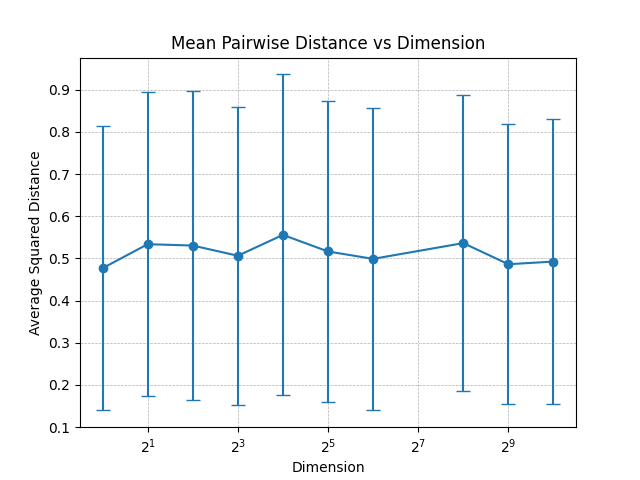
\includegraphics[width=\linewidth]{images/Figure_1_1c.png}
        \caption{Average distance between points in the unit cube.}
        \label{fig:average_distance}
    \end{minipage}
    \hspace{0.05\textwidth} % smaller gap
    \begin{minipage}[b]{0.4\textwidth}
        \centering
        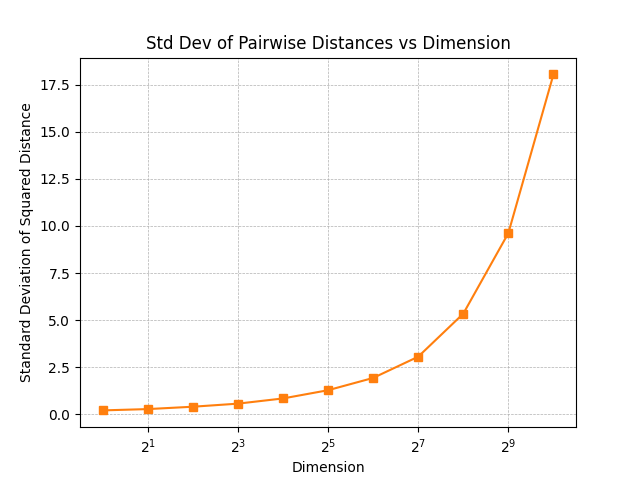
\includegraphics[width=\linewidth]{images/Figure_2_1c.png}
        \caption{Standard deviation of distance between points in the unit cube.}
        \label{fig:std_distance}
    \end{minipage}
\end{figure}

\color{black}
\subsection*{(d)}
\color{answer}
\textbf{Answer:}
I dont even know bro \\
\color{black}
\end{document}
